\documentclass{article}\usepackage{graphicx, color}
%% maxwidth is the original width if it is less than linewidth
%% otherwise use linewidth (to make sure the graphics do not exceed the margin)
\makeatletter
\def\maxwidth{ %
  \ifdim\Gin@nat@width>\linewidth
    \linewidth
  \else
    \Gin@nat@width
  \fi
}
\makeatother

\definecolor{fgcolor}{rgb}{0.2, 0.2, 0.2}
\newcommand{\hlnumber}[1]{\textcolor[rgb]{0,0,0}{#1}}%
\newcommand{\hlfunctioncall}[1]{\textcolor[rgb]{0.501960784313725,0,0.329411764705882}{\textbf{#1}}}%
\newcommand{\hlstring}[1]{\textcolor[rgb]{0.6,0.6,1}{#1}}%
\newcommand{\hlkeyword}[1]{\textcolor[rgb]{0,0,0}{\textbf{#1}}}%
\newcommand{\hlargument}[1]{\textcolor[rgb]{0.690196078431373,0.250980392156863,0.0196078431372549}{#1}}%
\newcommand{\hlcomment}[1]{\textcolor[rgb]{0.180392156862745,0.6,0.341176470588235}{#1}}%
\newcommand{\hlroxygencomment}[1]{\textcolor[rgb]{0.43921568627451,0.47843137254902,0.701960784313725}{#1}}%
\newcommand{\hlformalargs}[1]{\textcolor[rgb]{0.690196078431373,0.250980392156863,0.0196078431372549}{#1}}%
\newcommand{\hleqformalargs}[1]{\textcolor[rgb]{0.690196078431373,0.250980392156863,0.0196078431372549}{#1}}%
\newcommand{\hlassignement}[1]{\textcolor[rgb]{0,0,0}{\textbf{#1}}}%
\newcommand{\hlpackage}[1]{\textcolor[rgb]{0.588235294117647,0.709803921568627,0.145098039215686}{#1}}%
\newcommand{\hlslot}[1]{\textit{#1}}%
\newcommand{\hlsymbol}[1]{\textcolor[rgb]{0,0,0}{#1}}%
\newcommand{\hlprompt}[1]{\textcolor[rgb]{0.2,0.2,0.2}{#1}}%

\usepackage{framed}
\makeatletter
\newenvironment{kframe}{%
 \def\at@end@of@kframe{}%
 \ifinner\ifhmode%
  \def\at@end@of@kframe{\end{minipage}}%
  \begin{minipage}{\columnwidth}%
 \fi\fi%
 \def\FrameCommand##1{\hskip\@totalleftmargin \hskip-\fboxsep
 \colorbox{shadecolor}{##1}\hskip-\fboxsep
     % There is no \\@totalrightmargin, so:
     \hskip-\linewidth \hskip-\@totalleftmargin \hskip\columnwidth}%
 \MakeFramed {\advance\hsize-\width
   \@totalleftmargin\z@ \linewidth\hsize
   \@setminipage}}%
 {\par\unskip\endMakeFramed%
 \at@end@of@kframe}
\makeatother

\definecolor{shadecolor}{rgb}{.97, .97, .97}
\definecolor{messagecolor}{rgb}{0, 0, 0}
\definecolor{warningcolor}{rgb}{1, 0, 1}
\definecolor{errorcolor}{rgb}{1, 0, 0}
\newenvironment{knitrout}{}{} % an empty environment to be redefined in TeX

\usepackage{alltt}

\usepackage{xltxtra} %% For XeTeX font commands
\usepackage[includeheadfoot, margin = 0.5in]{geometry} %% Margins
\usepackage{hyperref}
\usepackage{graphicx} 
\usepackage{sectsty} %% Change format (font) of section headers
\usepackage{tikz}    %% Graphics for banner
\usepackage{parskip} %% Lines between paragraphs, no indentation
\usepackage{booktabs} %% Pretty up the tables
\usepackage[width = .5\textwidth]{caption} %% Width of captions
\usepackage{xcolor}

% \usepackage[normalem]{ulem} %% For underlines (in the URLs)
% \DeclareUrlCommand{\ulurl}{\uline}

%% Colors
\definecolor{pocDGreen}{HTML}{788172}
\definecolor{pocLGreen}{HTML}{A2B69A}
\definecolor{pocDBlue}{HTML}{3B6E8F}
\definecolor{pocLBlue}{HTML}{A3DCE6}
\definecolor{pocPurple}{HTML}{A784B4}

%% Fonts
\setmainfont{Frutiger LT Std 55 Roman}
\allsectionsfont{\fontspec{Archer}}

\usepackage{fancyhdr} %% Header and Footer formatting
\pagestyle{fancy}

%% Hyperlinks, PDF properties
\hypersetup{
    pdftitle = {POC County Report},
    pdfauthor = {Partners for Our Children},
    pdfcreator = {Gregor Passolt},
    pdfproducer = {Gregor Passolt},
    %hidelinks,
    unicode = true
}

% \makeatletter
% \DeclareUrlCommand\ULurl@@{%
%   %\def\UrlFont{\ttfamily\color{blue}}%
%   \def\UrlLeft{\uline\bgroup}%
%   \def\UrlRight{\egroup}}
% \def\ULurl@#1{\hyper@linkurl{\ULurl@@{#1}}{#1}}
% \DeclareRobustCommand*\ULurl{\hyper@normalise\ULurl@}
% \makeatother


%%% Header
\renewcommand{\sectionmark}[1]{\markboth{\MakeUppercase{#1}}{\MakeUppercase{#1}}}
\fancyhf{}
\renewcommand{\headrulewidth}{0.5pt}
\renewcommand{\headrule}{\hbox to\headwidth{%
\color{pocDGreen}\leaders\hrule height \headrulewidth\hfill}}
\rhead{\color{pocDGreen} \leftmark}

%%% Footer
\lfoot{\color{pocDGreen} \href{http://www.partnersforourchildren.org}{www.partnersforourchildren.org}}
\rfoot{\color{pocDGreen} \thepage}
\renewcommand{\footrulewidth}{0.5pt}
\renewcommand{\footrule}{\hbox to\headwidth{\color{pocDGreen}\leaders\hrule height \footrulewidth\hfill}}
\IfFileExists{upquote.sty}{\usepackage{upquote}}{}

\begin{document}
\frenchspacing %% Single space after period






\lhead{\color{pocDGreen} Pierce County Report}
\thispagestyle{empty} %% No header/footer on first page

%\vspace{-2in}

\begin{tikzpicture}[x=1in, y=1in]

    %%    Set up constants
    \def\banX{\textwidth}
    \def\banY{2.1in}
    \def\stripeHeight{0.5in}
    \def\stripeYpos{0.55in} %% From top
    \def\triX{0.25in}
    \def\triY{0.15in}
    \def\logoInsetX{0.7in}
    \def\logoInsetY{18pt}
    
    %% Draw Background Geomety
    \filldraw[pocLGreen] (0, 0) rectangle ++(\banX, \banY);
    \filldraw[pocDGreen] (0, \banY - \stripeYpos) rectangle ++(\banX + \triX, - \stripeHeight);
    \filldraw[fill=pocLGreen, draw=pocDGreen, join=bevel, thick]
        (\banX, \banY - \stripeYpos - \stripeHeight) -- ++(\triX, 0) -- ++(-\triX, -\triY) -- cycle;
    
    %% Above-stripe Text
    \node[pocDBlue, below left = 6pt, align = right] at (\banX, \banY)
        {\textbf{Automated County Report}\\\textbf{Generated \today}};
    \node at (\logoInsetX, \banY - \logoInsetY)
        {
\includegraphics[height=0.3in]{pocLogoSmall}};
    
    %% Stripe Text
    \node[right = 6pt, white] at (0, \banY - \stripeYpos - \stripeHeight + 16pt)
        {\fontspec{Archer}\Huge{Focus on Pierce County}};
    
    %% Below Stripe Text
    \node[below right = 6pt, pocDBlue, align = left, text width = \textwidth - 12pt]
        at (0, \banY - \stripeYpos - \stripeHeight - 3pt) {
         This \emph{Focus on Pierce County} report is one of a series of county-focused reports. The reports mirror the structure of the Child Well-Being Data Portal by providing information on three major parts of the child welfare system: Investigations \& Assessments, In-Home Services, and Out-of-Home Care. Each report is updated quarterly; check the Partners for Our Children webpage for the most recent version.
        If you are viewing this document on an Internet-connected device, light blue boxes indicate hyperlinks.} ;
    
\end{tikzpicture}

\vspace{-18pt}

\section*{Overview}

The Department of Social and Health Services (DSHS) divides Washington State into three regions. Pierce County is in Region~3, along with Clallam, Clark, Cowlitz, Grays Harbor, Jefferson, Kitsap, Lewis, Mason, Pacific, Pierce, Skamania, Thurston, and Wahkiakum counties.

As is done on the Data Portal, this report categorizes trends in Investigations \& Assessments and trends in In-Home Services by DCFS (Division of Children and Family Services) by offices and office groups, whereas trends in Out-of-Home Care are geographically categorized by county. 

\emph{County Focus} sections for Investigations \& Assessments and for In-Home Services display quarterly point-in-time (i.e., first day of the quarter) trend data for each DCFS office/office group in Pierce County. The \emph{County Focus} section for Out-of-Home Care shows quarterly point-in-time trend data for the entire county.

\emph{Region 3} sections feature "dotplots" that compare rates of Investigations \& Assessments and of In-Home Services per 1,000 households for all office/office groups in Pierce County. A third \emph{Region 3} section also provides a dotplot that compares rates of Out-of-Home Care per 1,000 children for each county in Region~3. Washington State is also included in the dotplots to give context to the rates presented in each regional section.  See \href{http://www.partnersforourchildren.org/publications/counts-vs-rates}{Technical Bulletin: The Difference Between Counts and Rates} for more information.

Table 1 provides relevant Census data for Pierce County and Washington State. Census data for the total population and for the number of children under 18 years of age are used in the calculation of the rates in the \emph{Region 3} sections below.

% latex table generated in R 3.0.0 by xtable 1.7-1 package
% Wed May 01 14:01:45 2013
\begin{table}[ht]
\centering
\caption{Pierce County Summary} 
\begin{tabular}{lrr}
  \toprule
 & Pierce County & Washington \\ 
  \midrule
Total population (2012) & 811,681 & 6,897,012 \\ 
  Percent change in population (2010 to 2012) & 2.1\% & 2.6\% \\ 
  Population under 5 years & 6.9\% & 6.5\% \\ 
  Population under 18 years & 24.3\% & 23.2\% \\ 
  Population: White alone & 77.3\% & 82.0\% \\ 
  Population: Black alone & 7.1\% & 3.8\% \\ 
  Population: American Indian/Alaska Native alone & 1.6\% & 1.8\% \\ 
  Population: Asian alone & 6.2\% & 7.5\% \\ 
  Population: Native Hawaiian/Other Pacific Islander alone & 1.4\% & 0.7\% \\ 
  Population: Multiracial & 6.4\% & 4.3\% \\ 
  Population: Hispanic or Latino Origin & 9.4\% & 11.6\% \\ 
  Population: Not Hispanic, White alone & 70.1\% & 72.1\% \\ 
  Education: High school graduate (age $>$25) & 90.1\% & 89.8\% \\ 
  People below poverty line (all ages) & 11.6\% & 12.5\% \\ 
  Population per square mile & 476.3 & 101.2 \\ 
   \bottomrule
\end{tabular}
\end{table}



\section{\href{http://www.partnersforourchildren.org//child-well-being/visualizations/investigations-assessments/trends}
{Investigations \& Assessments}}
When professionals and community members report suspected instances of child abuse or neglect to the child welfare system, some of the reports are investigated, some are assessed only (e.g., Family Reconciliation Services), and some \emph{screened out} because the information reported (if true) does not meet the statutory definition of child abuse or neglect and there is no need for an assessment.

\subsection{\href{http://www.partnersforourchildren.org//child-well-being/visualizations/investigations-assessments/trends}
{Investigations \& Assessments:} Pierce County Focus}
The following graphs indicate recent trends in Investigations \& Assessments for the two DCFS offices/office groups in Pierce County.
Data are presented using "unduplicated counts" (see \href{http://http://www.partnersforourchildren.org/publications/using-different-count-types-data-portal}{Technical Bulletin: Interpreting the Type of Count Filter} for more information).  
\nopagebreak[2]
\begin{knitrout}
\definecolor{shadecolor}{rgb}{0.969, 0.969, 0.969}\color{fgcolor}

{\centering 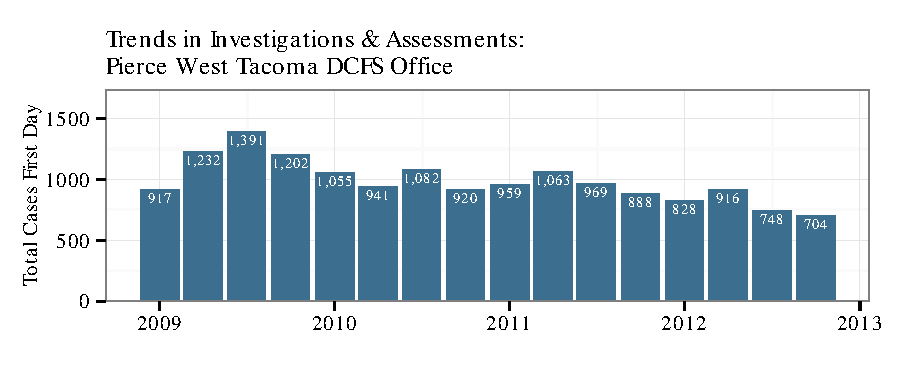
\includegraphics[width=\maxwidth]{figure/ia_focus1} 
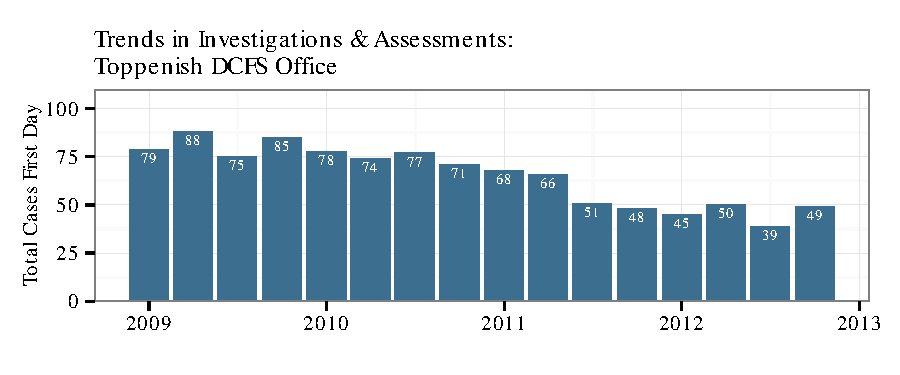
\includegraphics[width=\maxwidth]{figure/ia_focus2} 

}



\end{knitrout}




\subsection{
    \href{http://www.partnersforourchildren.org//child-well-being/visualizations/investigations-assessments/trends}
    {Investigations \& Assessment: Region 3}}
To give context to the trend data, the following plot shows the rate of Investigations \& Assessments for Quarter 4, 2012 for Region~3 office groups and all of Washington State.
\nopagebreak[3]
\begin{knitrout}
\definecolor{shadecolor}{rgb}{0.969, 0.969, 0.969}\color{fgcolor}

{\centering 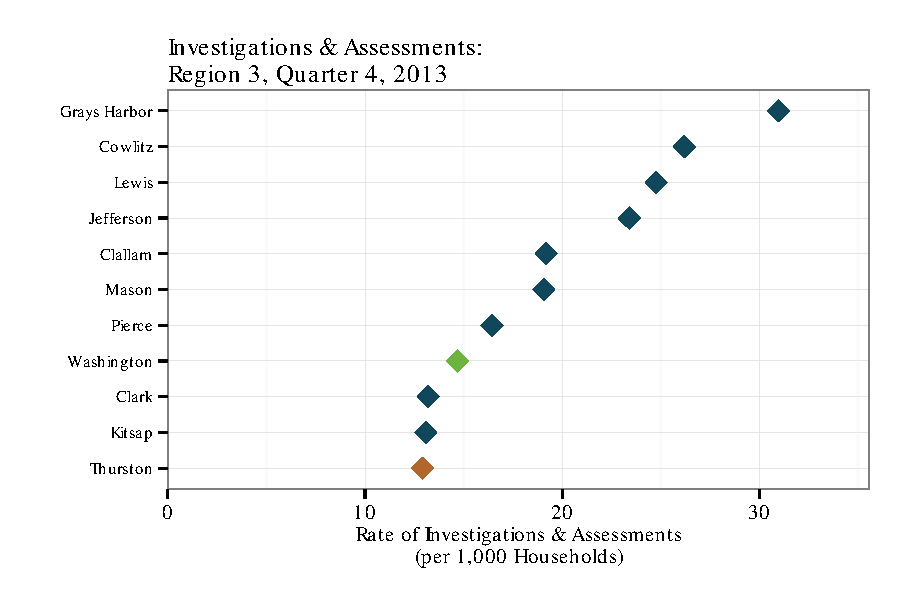
\includegraphics[width=\maxwidth]{figure/ia_context} 

}



\end{knitrout}



%%%%%%%%%%%%%%%%%%%%%%%%%%%%%%%%%%%%%%%%%%%%%%%% ----
\section{\href{http://www.partnersforourchildren.org/child-well-being/visualizations/home-services/trends}
    {In-Home Services}
}
When an investigation identifies a threat to a child's safety, case workers will first determine if the child can be kept safely at home through a safety plan. If so, the family and child may be provided with various services that range from concrete support (e.g., food, appliance repair, etc.) to referrals to community services (e.g., drug and alcohol assessments, etc.).


\subsection{\href{http://www.partnersforourchildren.org/child-well-being/visualizations/home-services/trends}
    {In-Home Services: Pierce County Focus}
}
The following graphs show the recent trends in In-Home Services for the two DCFS offices in
Pierce County.
Data are presented using "unduplicated counts" (see \href{http://http://www.partnersforourchildren.org/publications/using-different-count-types-data-portal}{Technical Bulletin: Interpreting the Type of Count Filter} for more information). 
\nopagebreak[3]
\begin{knitrout}
\definecolor{shadecolor}{rgb}{0.969, 0.969, 0.969}\color{fgcolor}

{\centering 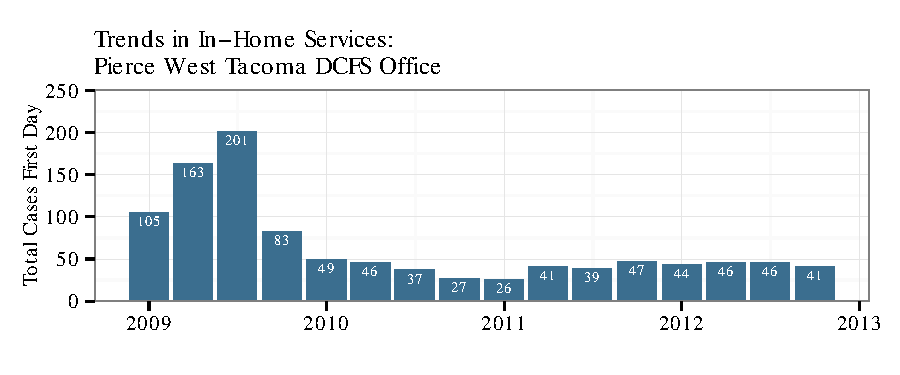
\includegraphics[width=\maxwidth]{figure/ihs_focus1} 
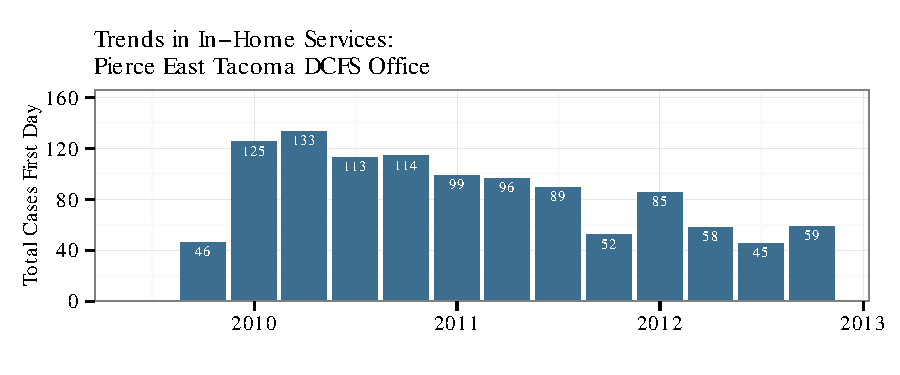
\includegraphics[width=\maxwidth]{figure/ihs_focus2} 

}



\end{knitrout}




\subsection{\href{http://www.partnersforourchildren.org/child-well-being/visualizations/home-services/trends}
    {In-Home Services:} Region 3
}
To give context to the trend data above, the following plot shows the rate of In-Home Services for Quarter 4, 2012 for Region~3 offices and all of Washington State.
\nopagebreak[3]
\begin{knitrout}
\definecolor{shadecolor}{rgb}{0.969, 0.969, 0.969}\color{fgcolor}

{\centering 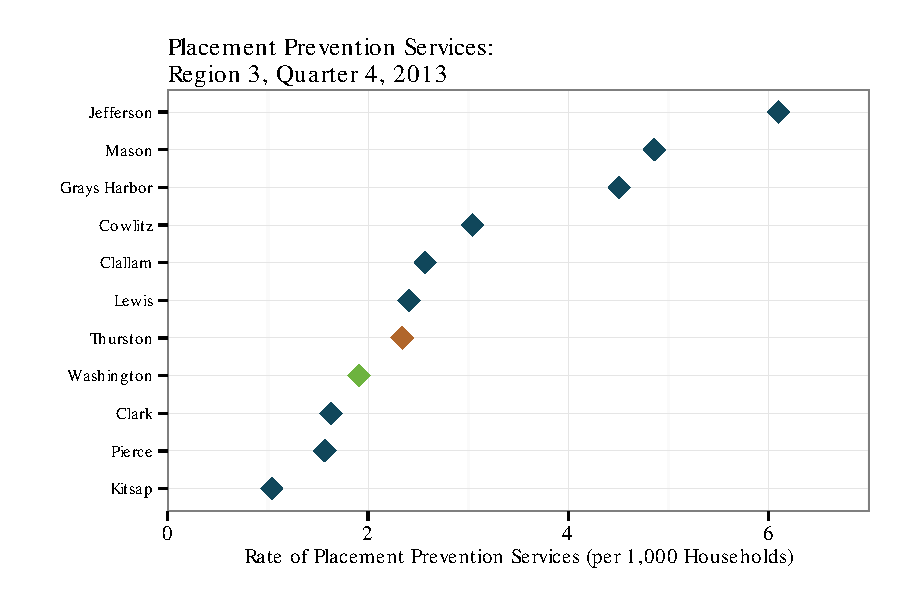
\includegraphics[width=\maxwidth]{figure/ihs_context} 

}



\end{knitrout}



\subsection{\href{http://www.partnersforourchildren.org/child-well-being/visualizations/home-services/safety}
    {In-Home Services: Safety}
}
At times the in-home services provided to families do not, or cannot, adequately address the issues identified during the investigation. Other times, new issues are raised during the course of an in-home services case. Either way, when the case worker decides that it is not possible for the child to remain safely in their home, steps will be taken to place the child in out-of-home care.

The measurements in Table 2 identify placement into Out-of-Home Care among families and their children who have received In-Home Services for one year and for two years. If the in-home services are completed effectively, and/or circumstances become such that the child can remain in-home safely, there should be no need to place the child in out-of-home care. Thus, in general, the lower percentages indicate better outcomes.

% latex table generated in R 3.0.0 by xtable 1.7-1 package
% Wed May 01 14:01:47 2013
\begin{table}[ht]
\centering
\caption{Percent of In-Home Service Cases Resulting in Out-of-Home Care Placement.} 
\begin{tabular}{lrr}
  \toprule
 & Within 1 Year & Within 2 Years \\ 
  \midrule
WASHINGTON & 18\% & 20\% \\ 
  Pierce West Tacoma & 21\% & 25\% \\ 
  Pierce East Tacoma & 23\% & 24\% \\ 
   \bottomrule
\end{tabular}
\end{table}



%%%%%%%%%%%%%%%%%%%%%%%%%%%%%%%%%%%%%%%%%%%%%%%%% ----
\section{\href{http://www.partnersforourchildren.org/child-well-being/visualizations/out-home-care/trends}
    {Out-of-Home Care}
}
When children cannot remain safely in their home, they are placed in out-of-home care. Once a child is removed, the child welfare system works to find a safe and permanent home for the child. Most children ultimately reunify with their parents after all safety conerns have been addressed; however, some children exit to other permanency outcomes (e.g., adoption, guardianship, etc.).

Note that Garfield, Lincoln, San Juan, Wahkiakum, Skamania, and Columbia Counties are omitted from comparisons in the Out-of-Home Care section due to a small number of out-of-home placements.

\subsection{\href{http://www.partnersforourchildren.org/child-well-being/visualizations/out-home-care/trends}
 {Out-of-Home Care: Pierce County Focus}
}
The following graph shows the recent trends in Out-of-Home Care for
Pierce County. Data are presented using "unduplicated counts" (see \href{http://http://www.partnersforourchildren.org/publications/using-different-count-types-data-portal}{Technical Bulletin: Interpreting the Type of Count Filter} for more information). 
\nopagebreak[3]
\begin{knitrout}
\definecolor{shadecolor}{rgb}{0.969, 0.969, 0.969}\color{fgcolor}

{\centering 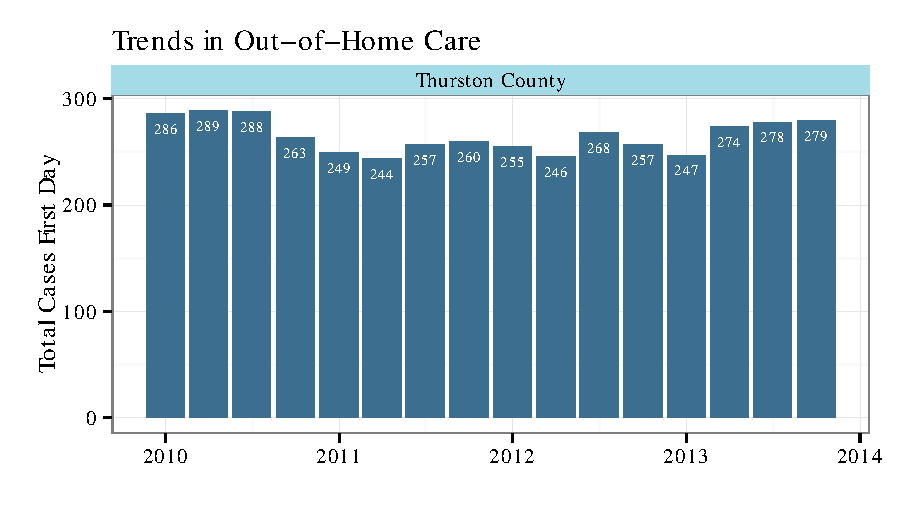
\includegraphics[width=\maxwidth]{figure/ooh_focus} 

}



\end{knitrout}


\subsection{\href{http://www.partnersforourchildren.org/child-well-being/visualizations/out-home-care/trends}
    {Out-of-Home Care: Region 3}
}
To give context to the trend data above, the following plot shows the rate of Out-of-Home Care for Quarter 4, 2012 for Region~3 counties and all of Washington.
\nopagebreak[3]
\begin{knitrout}
\definecolor{shadecolor}{rgb}{0.969, 0.969, 0.969}\color{fgcolor}

{\centering 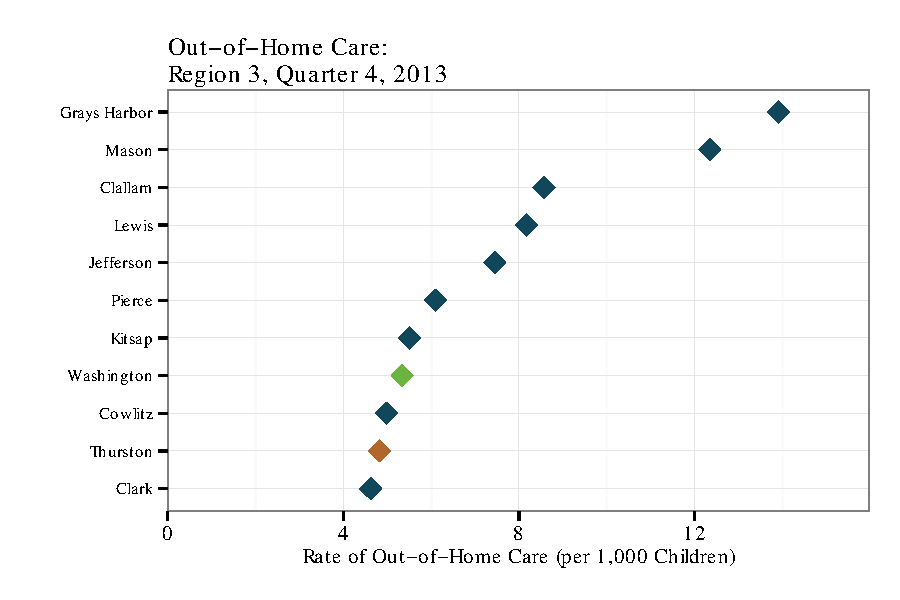
\includegraphics[width=\maxwidth]{figure/ooh_context} 

}



\end{knitrout}


\subsection{\href{http://www.partnersforourchildren.org/child-well-being/visualizations/out-home-care/safety}
    {Out-of-Home Care: Safety}
}

Sometimes, when children experience a given permanency outcome (e.g., reunification, guardianship, adoption), safety concerns resurface in the child's home. In such circumstances, these safety concerns can be severe enough that the child needs to re-enter out-of-home care.

Table 3 identifies the percentage of children re-entering out-of-home care within two years of discharge, by discharge type, for all of the counties in Region~3, as well as for Washington State overall. The higher percentages of re-entry point to the challenges of providing a safe permanent placement for the child.
\nopagebreak[3]
% latex table generated in R 3.0.0 by xtable 1.7-1 package
% Wed May 01 14:01:47 2013
\begin{table}[ht]
\centering
\caption{Percentage of Children Re-Entering Out-of-Home Care within Two Years of Discharge} 
\begin{tabular}{lrrr}
  \toprule
 & Reunification & Adoption & Guardianship \\ 
  \midrule
Jefferson & 37.5\% & 0\% & 0\% \\ 
  Clallam & 31.8\% & 0\% & 0\% \\ 
  Thurston & 22.2\% & 1.9\% & 11.1\% \\ 
  Pacific & 16.7\% & 0\% & 0\% \\ 
  Grays Harbor & 15\% & 0\% & 0\% \\ 
  Pierce & 13.2\% & 2.1\% & 1.1\% \\ 
  Clark & 13.1\% & 1.8\% & 4.3\% \\ 
  WASHINGTON & 12.8\% & 1.5\% & 5.7\% \\ 
  Kitsap & 9.7\% & 0\% & 27.3\% \\ 
  Mason & 8.8\% & 0\% & 0\% \\ 
  Cowlitz & 6.9\% & 0\% & 0\% \\ 
  Lewis & 6.5\% & 0\% & 33.3\% \\ 
   \bottomrule
\end{tabular}
\end{table}


In the table, "NA" indicates that no children in the cohort exited to that discharge type, whereas "0\%" indicates that children did exit to that discharge type, but none re-entered care.

%% Outcomes Chunk
\subsection{\href{http://www.partnersforourchildren.org/child-well-being/visualizations/out-home-care/outcomes}
    {Out-of-Home Care: Outcomes}
}
Under the Adoption and Safe Families Act of 1997 (ASFA), the goal of the child welfare system is to ensure that children are placed in safe and permanent homes as quickly as possible. The child welfare system seeks to first reunify children with their families when it is safe to do so. If children are unable to be safely reunified, permanency is achieved through adoption or guardianship. Some children exit from the system for other reasons such as emancipation or transfer of custody to different jurisdictions.

The following bar graph shows the percentage of children in the 2010 entry cohort achieving each outcome for Pierce County, Region~3, and Washington State.
\nopagebreak[3]
\begin{knitrout}
\definecolor{shadecolor}{rgb}{0.969, 0.969, 0.969}\color{fgcolor}

{\centering 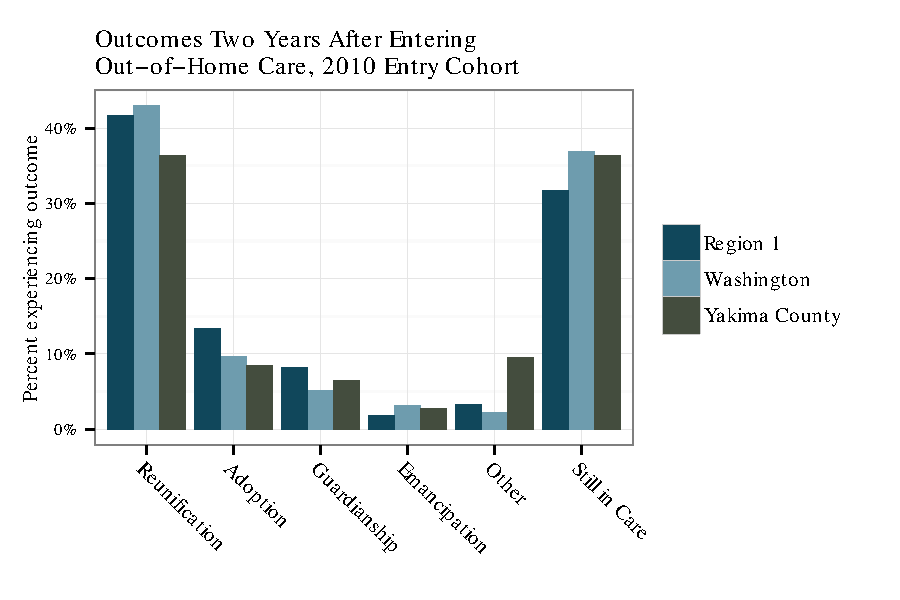
\includegraphics[width=\maxwidth]{figure/ooh_outcomes} 

}



\end{knitrout}


%% Well-Being
\subsection{\href{http://www.partnersforourchildren.org/child-well-being/visualizations/out-home-care/well-being}
    {Out-of-Home Care: Well-Being}
}

When placement in out-of-home care is necessary, the physical and psychological needs and well-being of the child must be considered. While individual needs vary, and well-being is difficult to measure directly, research has shown that placement with siblings and placement in kinship care enhances a child's physical and emotional health. Yet, in some cases, the child's best interests necessitate placement separate from their sibling(s) or in a non-family setting. For example, a sibling with physical, emotional, or mental conditions may require specialized services in order to accomplish specific therapeutic goals. In such cases, siblings may be separated and/or a child may be placed in a non-family setting until those therapeutic goals are met.

As a summary measurement of child well-being, the next graph shows the percent of care-days spent in kinship care for the counties in Region~3 from 2008 to 2012.
\nopagebreak[3]
\begin{knitrout}
\definecolor{shadecolor}{rgb}{0.969, 0.969, 0.969}\color{fgcolor}

{\centering 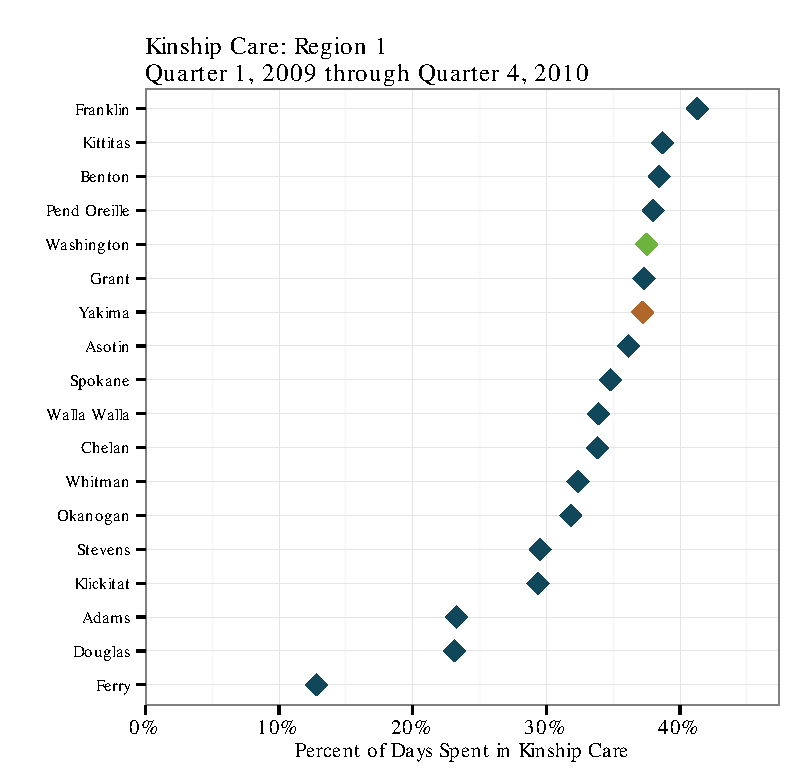
\includegraphics[width=\maxwidth]{figure/ooh_wb} 

}



\end{knitrout}



\end{document}

